% =====================================================================
%  Weight x KV-Cache Joint Quantization  --  Two-Stage Decomposition
%  Wide (landscape) pipeline figure for the paper.
%
%  COMPILE (standalone, pure TikZ -- no pgfplots needed):
%     pdflatex joint_search_figure.tex        % -> joint_search_figure.pdf (tight crop)
%
%  EMBED in a two-column paper:
%     \begin{figure*}[t]
%       \centering
%       \resizebox{\textwidth}{!}{\input{joint_search_figure_body.tex}}  % or \includegraphics of the pdf
%       \caption{...}\label{fig:joint}
%     \end{figure*}
%  (To reuse the body, move everything between \begin{tikzpicture}..\end{tikzpicture}
%   into joint_search_figure_body.tex and \input it.)
%
%  Color code (kept consistent across all panels):
%     W  axis / weight quant  = blue   (Wcol)
%     KV axis / kv-cache quant = orange (KVcol)
%     joint / Stage-2 output   = purple (Jcol)
%     infeasible / naive cost  = red    (badcol)
% =====================================================================
\documentclass[border=8pt]{standalone}
\usepackage{amsmath}
\usepackage{amssymb}   % \circlearrowright
\usepackage{tikz}
\usetikzlibrary{positioning,arrows.meta,fit,backgrounds,calc,shapes.geometric}

\definecolor{Wcol}{RGB}{31,119,180}    % blue  -- weight axis
\definecolor{KVcol}{RGB}{230,126,34}   % orange-- kv axis
\definecolor{Jcol}{RGB}{142,68,173}    % purple-- joint / ours
\definecolor{badcol}{RGB}{200,40,40}   % red   -- naive / infeasible
\definecolor{goodcol}{RGB}{39,140,70}  % green -- cheap cost

% ---- mini Pareto-front glyph: convex-decreasing curve + scatter ------
% #1 = color, #2 = x-axis label, #3 = y-axis label. Drawn at local (0,0).
\newcommand{\paretomini}[3]{%
  \draw[-{Stealth[length=1.6mm]},gray!70] (0,0) -- (2.35,0)
        node[below=0pt,font=\tiny,text=black]{#2};
  \draw[-{Stealth[length=1.6mm]},gray!70] (0,0) -- (0,1.7);
  \node[font=\tiny,rotate=90,anchor=south] at (-0.12,0.85) {#3};
  \draw[#1,line width=1pt]
     (0.18,1.5) .. controls (0.55,0.55) and (1.2,0.4) .. (2.15,0.28);
  \foreach \px/\py in {0.22/1.45,0.5/0.78,0.82/0.52,1.2/0.4,1.6/0.32,2.05/0.28}
     \fill[#1] (\px,\py) circle (1.5pt);
}

% ---- one stacked "block library" shelf -------------------------------
% #1 = color, #2 = title, #3/#4/#5/#6 = four block captions (bit values)
\newcommand{\shelf}[6]{%
  \node[font=\scriptsize\bfseries,text=#1] at (0,1.05) {#2};
  \foreach \i/\lab [count=\k from 0] in {0/#3,1/#4,2/#5,3/#6}{
     \node[draw=#1,fill=#1!12,rounded corners=1.5pt,minimum width=0.9cm,
           minimum height=0.5cm,font=\tiny] at (\k*1.0,0.35) {\lab};
  }
}

\begin{document}
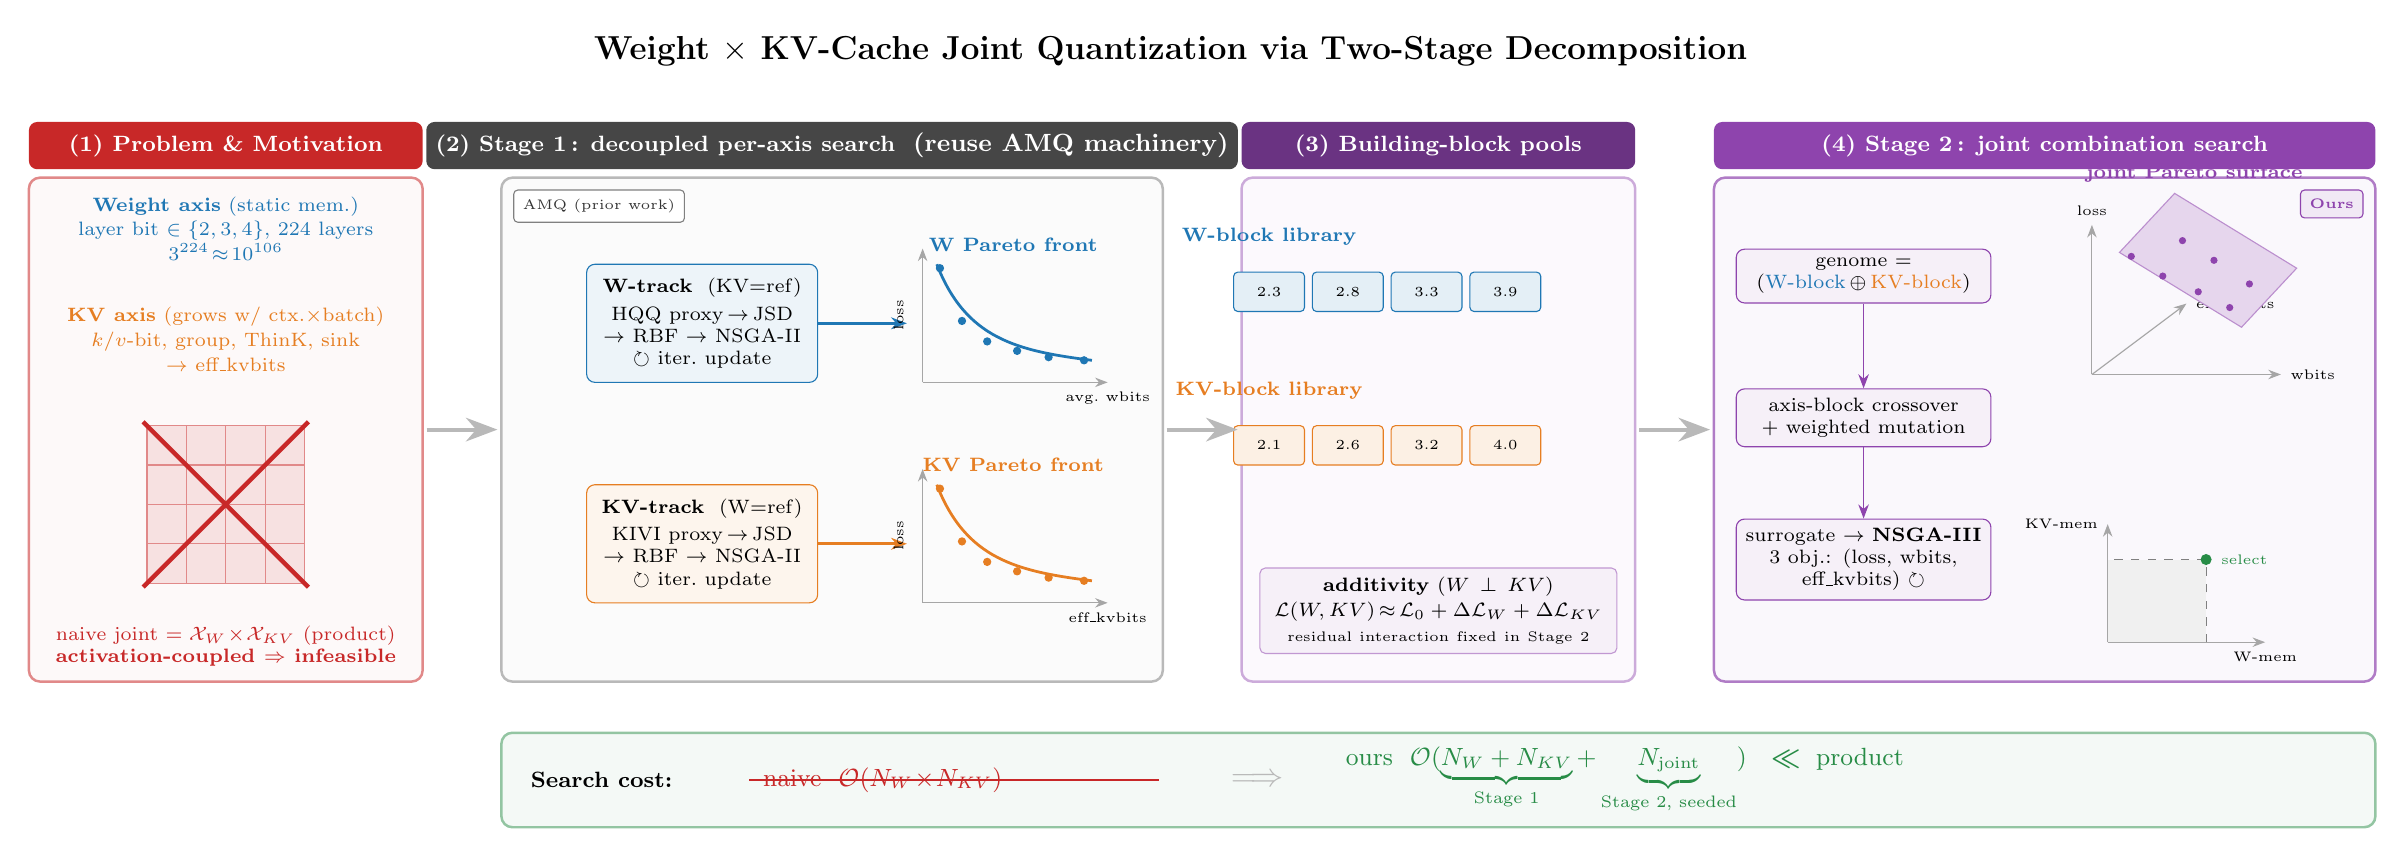
\begin{tikzpicture}[font=\sffamily]

% ============ global title ============================================
\node[font=\large\bfseries] at (14.5,8.0)
   {Weight $\times$ KV-Cache Joint Quantization via Two-Stage Decomposition};

% helper: panel body + header chip  (macro-free, drawn per panel below)
% panel body y in [0,6.4]; header chip sits at y=6.75

% ==================================================================== %
%  PANEL (1)  Problem & Motivation           x in [0,5.0]              %
% ==================================================================== %
\begin{scope}
  \draw[rounded corners=4pt,draw=badcol!55,fill=badcol!3,line width=0.9pt]
        (0,0) rectangle (5.0,6.4);
  \node[rounded corners=3pt,fill=badcol,text=white,font=\footnotesize\bfseries,
        minimum width=5.0cm,minimum height=0.6cm,anchor=south] at (2.5,6.5)
        {(1) Problem \& Motivation};

  \node[align=center,font=\scriptsize,text=Wcol] at (2.5,5.75)
        {\textbf{Weight axis} (static mem.)\\[1pt]
         layer bit $\in\{2,3,4\}$,\ 224 layers\\[1pt] $3^{224}\!\approx\!10^{106}$};
  \node[align=center,font=\scriptsize,text=KVcol] at (2.5,4.35)
        {\textbf{KV axis} (grows w/ ctx.$\times$batch)\\[1pt]
         $k/v$-bit, group, ThinK, sink\\[1pt] $\to$ eff\_kvbits};

  % product grid
  \begin{scope}[shift={(1.5,1.25)}]
     \foreach \gx in {0,...,3}{\foreach \gy in {0,...,3}{
        \draw[draw=badcol!55,fill=badcol!14] (\gx*0.5,\gy*0.5) rectangle (\gx*0.5+0.5,\gy*0.5+0.5);}}
     % big cross
     \draw[badcol,line width=1.6pt] (-0.05,-0.05) -- (2.05,2.05);
     \draw[badcol,line width=1.6pt] (-0.05,2.05) -- (2.05,-0.05);
  \end{scope}
  \node[font=\scriptsize,align=center,text=badcol] at (2.5,0.45)
        {naive joint $=\mathcal{X}_W\!\times\!\mathcal{X}_{KV}$ (product)\\
         \textbf{activation-coupled $\Rightarrow$ infeasible}};
\end{scope}

% ==================================================================== %
%  PANEL (2)  Stage 1 -- decoupled per-axis search   x in [6.0,14.4]   %
% ==================================================================== %
\begin{scope}
  \draw[rounded corners=4pt,draw=gray!55,fill=gray!3,line width=0.9pt]
        (6.0,0) rectangle (14.4,6.4);
  \node[rounded corners=3pt,fill=gray!55!black,text=white,font=\footnotesize\bfseries,
        minimum width=8.4cm,minimum height=0.6cm,anchor=south] at (10.2,6.5)
        {(2) Stage 1\,: decoupled per-axis search \ \small(reuse AMQ machinery)};
  \node[draw=gray,fill=white,rounded corners=1.5pt,font=\tiny,text=gray!40!black,
        anchor=north west] at (6.15,6.25) {AMQ (prior work)};

  % --- top: W-track ---
  \node[draw=Wcol,rounded corners=3pt,fill=Wcol!8,align=center,font=\scriptsize,
        text width=2.7cm,minimum height=1.5cm] (amqW) at (8.55,4.55)
        {\textbf{W-track}\ \ (KV$=$ref)\\[2pt]
         HQQ proxy $\!\to\!$ JSD\\ $\to$ RBF $\to$ NSGA-II\\ $\circlearrowright$ iter.\ update};
  \draw[-{Stealth[length=2mm]},Wcol,line width=1pt] (amqW.east) -- (11.15,4.55);
  \begin{scope}[shift={(11.35,3.8)}] \paretomini{Wcol}{avg.\ wbits}{loss} \end{scope}
  \node[font=\scriptsize\bfseries,text=Wcol] at (12.5,5.55) {W Pareto front};

  % --- bottom: KV-track ---
  \node[draw=KVcol,rounded corners=3pt,fill=KVcol!8,align=center,font=\scriptsize,
        text width=2.7cm,minimum height=1.5cm] (amqK) at (8.55,1.75)
        {\textbf{KV-track}\ \ (W$=$ref)\\[2pt]
         KIVI proxy $\!\to\!$ JSD\\ $\to$ RBF $\to$ NSGA-II\\ $\circlearrowright$ iter.\ update};
  \draw[-{Stealth[length=2mm]},KVcol,line width=1pt] (amqK.east) -- (11.15,1.75);
  \begin{scope}[shift={(11.35,1.0)}] \paretomini{KVcol}{eff\_kvbits}{loss} \end{scope}
  \node[font=\scriptsize\bfseries,text=KVcol] at (12.5,2.75) {KV Pareto front};
\end{scope}

% ==================================================================== %
%  PANEL (3)  Block pools                          x in [15.4,20.4]    %
% ==================================================================== %
\begin{scope}
  \draw[rounded corners=4pt,draw=Jcol!45,fill=Jcol!3,line width=0.9pt]
        (15.4,0) rectangle (20.4,6.4);
  \node[rounded corners=3pt,fill=Jcol!75!black,text=white,font=\footnotesize\bfseries,
        minimum width=5.0cm,minimum height=0.6cm,anchor=south] at (17.9,6.5)
        {(3) Building-block pools};

  \begin{scope}[shift={(15.75,4.6)}]
     \shelf{Wcol}{W-block library}{2.3}{2.8}{3.3}{3.9}
  \end{scope}
  \begin{scope}[shift={(15.75,2.65)}]
     \shelf{KVcol}{KV-block library}{2.1}{2.6}{3.2}{4.0}
  \end{scope}

  % additivity inset (theoretical license for decomposition)
  \node[draw=Jcol!55,fill=Jcol!8,rounded corners=2pt,align=center,font=\scriptsize,
        text width=4.3cm] at (17.9,0.9)
        {\textbf{additivity} ($W\!\perp\!KV$)\\[1pt]
         $\mathcal{L}(W,KV)\!\approx\!\mathcal{L}_0+\Delta\mathcal{L}_W+\Delta\mathcal{L}_{KV}$\\[1pt]
         {\tiny residual interaction fixed in Stage 2}};
\end{scope}

% ==================================================================== %
%  PANEL (4)  Stage 2 -- joint combination search   x in [21.4,29.8]   %
% ==================================================================== %
\begin{scope}
  \draw[rounded corners=4pt,draw=Jcol!70,fill=Jcol!4,line width=0.9pt]
        (21.4,0) rectangle (29.8,6.4);
  \node[rounded corners=3pt,fill=Jcol,text=white,font=\footnotesize\bfseries,
        minimum width=8.4cm,minimum height=0.6cm,anchor=south] at (25.6,6.5)
        {(4) Stage 2\,: joint combination search};
  \node[draw=Jcol,fill=Jcol!12,rounded corners=1.5pt,font=\tiny\bfseries,text=Jcol,
        anchor=north east] at (29.65,6.25) {Ours};

  \node[draw=Jcol,rounded corners=3pt,fill=Jcol!8,align=center,font=\scriptsize,
        text width=3.0cm] (gen) at (23.3,5.15)
        {genome $=$\\ (\textcolor{Wcol}{W-block}\,$\oplus$\,\textcolor{KVcol}{KV-block})};
  \node[draw=Jcol,rounded corners=3pt,fill=Jcol!8,align=center,font=\scriptsize,
        text width=3.0cm] (ops) at (23.3,3.35)
        {axis-block crossover\\ $+$ weighted mutation};
  \node[draw=Jcol,rounded corners=3pt,fill=Jcol!8,align=center,font=\scriptsize,
        text width=3.0cm] (nsga) at (23.3,1.55)
        {surrogate $\to$ \textbf{NSGA-III}\\ 3 obj.: (loss, wbits,\\ eff\_kvbits) $\circlearrowright$};
  \draw[-{Stealth[length=1.8mm]},Jcol] (gen) -- (ops);
  \draw[-{Stealth[length=1.8mm]},Jcol] (ops) -- (nsga);

  % 3D-ish joint Pareto surface
  \begin{scope}[shift={(26.2,3.9)}]
     \draw[-{Stealth[length=1.6mm]},gray!70] (0,0) -- (2.4,0) node[right,font=\tiny,text=black]{wbits};
     \draw[-{Stealth[length=1.6mm]},gray!70] (0,0) -- (0,1.9) node[above,font=\tiny,text=black]{loss};
     \draw[-{Stealth[length=1.6mm]},gray!70] (0,0) -- (1.2,0.9) node[right,font=\tiny,text=black]{eff\_kvbits};
     \fill[Jcol!22,draw=Jcol!60] (0.35,1.55) -- (1.9,0.6) -- (2.6,1.35) -- (1.05,2.3) -- cycle;
     \foreach \px/\py in {0.5/1.5,0.9/1.25,1.35/1.05,1.75/0.85,1.15/1.7,1.55/1.45,2.0/1.15}
        \fill[Jcol] (\px,\py) circle (1.3pt);
     \node[font=\scriptsize\bfseries,text=Jcol] at (1.3,2.55) {joint Pareto surface};
  \end{scope}

  % 2D deployment budget box
  \begin{scope}[shift={(26.4,0.5)}]
     \draw[-{Stealth[length=1.6mm]},gray!70] (0,0) -- (2.0,0) node[below,font=\tiny,text=black]{W-mem};
     \draw[-{Stealth[length=1.6mm]},gray!70] (0,0) -- (0,1.5) node[left,font=\tiny,text=black]{KV-mem};
     \draw[dashed,gray] (1.25,0) -- (1.25,1.05) -- (0,1.05);
     \fill[gray!12] (0,0) rectangle (1.25,1.05);
     \fill[goodcol] (1.25,1.05) circle (2pt);
     \node[font=\tiny,text=goodcol,anchor=west] at (1.32,1.05) {select};
  \end{scope}
\end{scope}

% ==================================================================== %
%  big inter-panel pipeline arrows                                     %
% ==================================================================== %
\foreach \xa/\xb in {5.05/5.95, 14.45/15.35, 20.45/21.35}
   \draw[-{Stealth[length=4mm]},line width=1.4pt,gray!55] (\xa,3.2) -- (\xb,3.2);

% ==================================================================== %
%  bottom COST ribbon  (spans Stage 1..2)                              %
% ==================================================================== %
\begin{scope}
  \draw[rounded corners=4pt,draw=goodcol!50,fill=goodcol!5,line width=0.9pt]
        (6.0,-1.85) rectangle (29.8,-0.65);
  \node[font=\footnotesize\bfseries,anchor=west] at (6.25,-1.25) {Search cost:};
  \node[font=\small,text=badcol,anchor=west] at (9.2,-1.25)
        {naive $\ \mathcal{O}(N_W\!\times\!N_{KV})$};
  \draw[badcol,line width=1pt] (9.15,-1.25) -- (14.35,-1.25); % strike-through
  \node[font=\large,text=gray!55] at (15.6,-1.25) {$\Longrightarrow$};
  \node[font=\small,text=goodcol,anchor=west] at (16.6,-1.25)
        {ours $\ \mathcal{O}(\underbrace{N_W+N_{KV}}_{\text{Stage 1}}+\underbrace{N_{\text{joint}}}_{\text{Stage 2, seeded}})\ \ \boldsymbol{\ll}\ \text{product}$};
\end{scope}

\end{tikzpicture}
\end{document}
